\documentclass[10pt]{amsart}
\usepackage[margin=1.4in]{geometry}
\usepackage{amssymb,amsmath,enumitem,url, bm}
\usepackage{graphicx,subfig}
\graphicspath{ {./images/} }
\usepackage{cancel}

\newcommand{\D}{\mathrm{d}}
\newcommand{\I}{\mathrm{i}}
\DeclareMathOperator{\E}{e}
\DeclareMathOperator{\OO}{O}
\DeclareMathOperator{\oo}{o}
\DeclareMathOperator{\erfc}{erfc}
\DeclareMathOperator{\real}{Re}
\DeclareMathOperator{\imag}{Im}
\usepackage{tikz}
\usepackage[framemethod=tikz]{mdframed}
\theoremstyle{nonumberplain}

\mdtheorem[innertopmargin=-5pt]{sol}{Solution}
%\newmdtheoremenv[innertopmargin=-5pt]{sol}{Solution}

\begin{document}
\pagestyle{empty}

\newcommand{\mline}{\vspace{.2in}\hrule\vspace{.2in}}

\noindent
\text{Hunter Lybbert} \\
\text{Student ID: 2426454} \\
\text{04-21-25} \\
\text{HMS 581} \\
% header containing your name, student number, due date, course, and the homework number as a title.

\title{\bf {Homework 2} }


\maketitle
\noindent
This document contains Figures produced when running the simulations for homework 2.
In the future a comments and observations may be added but for now this is just the results only.
\mline

\begin{figure}[h]
	\centering
	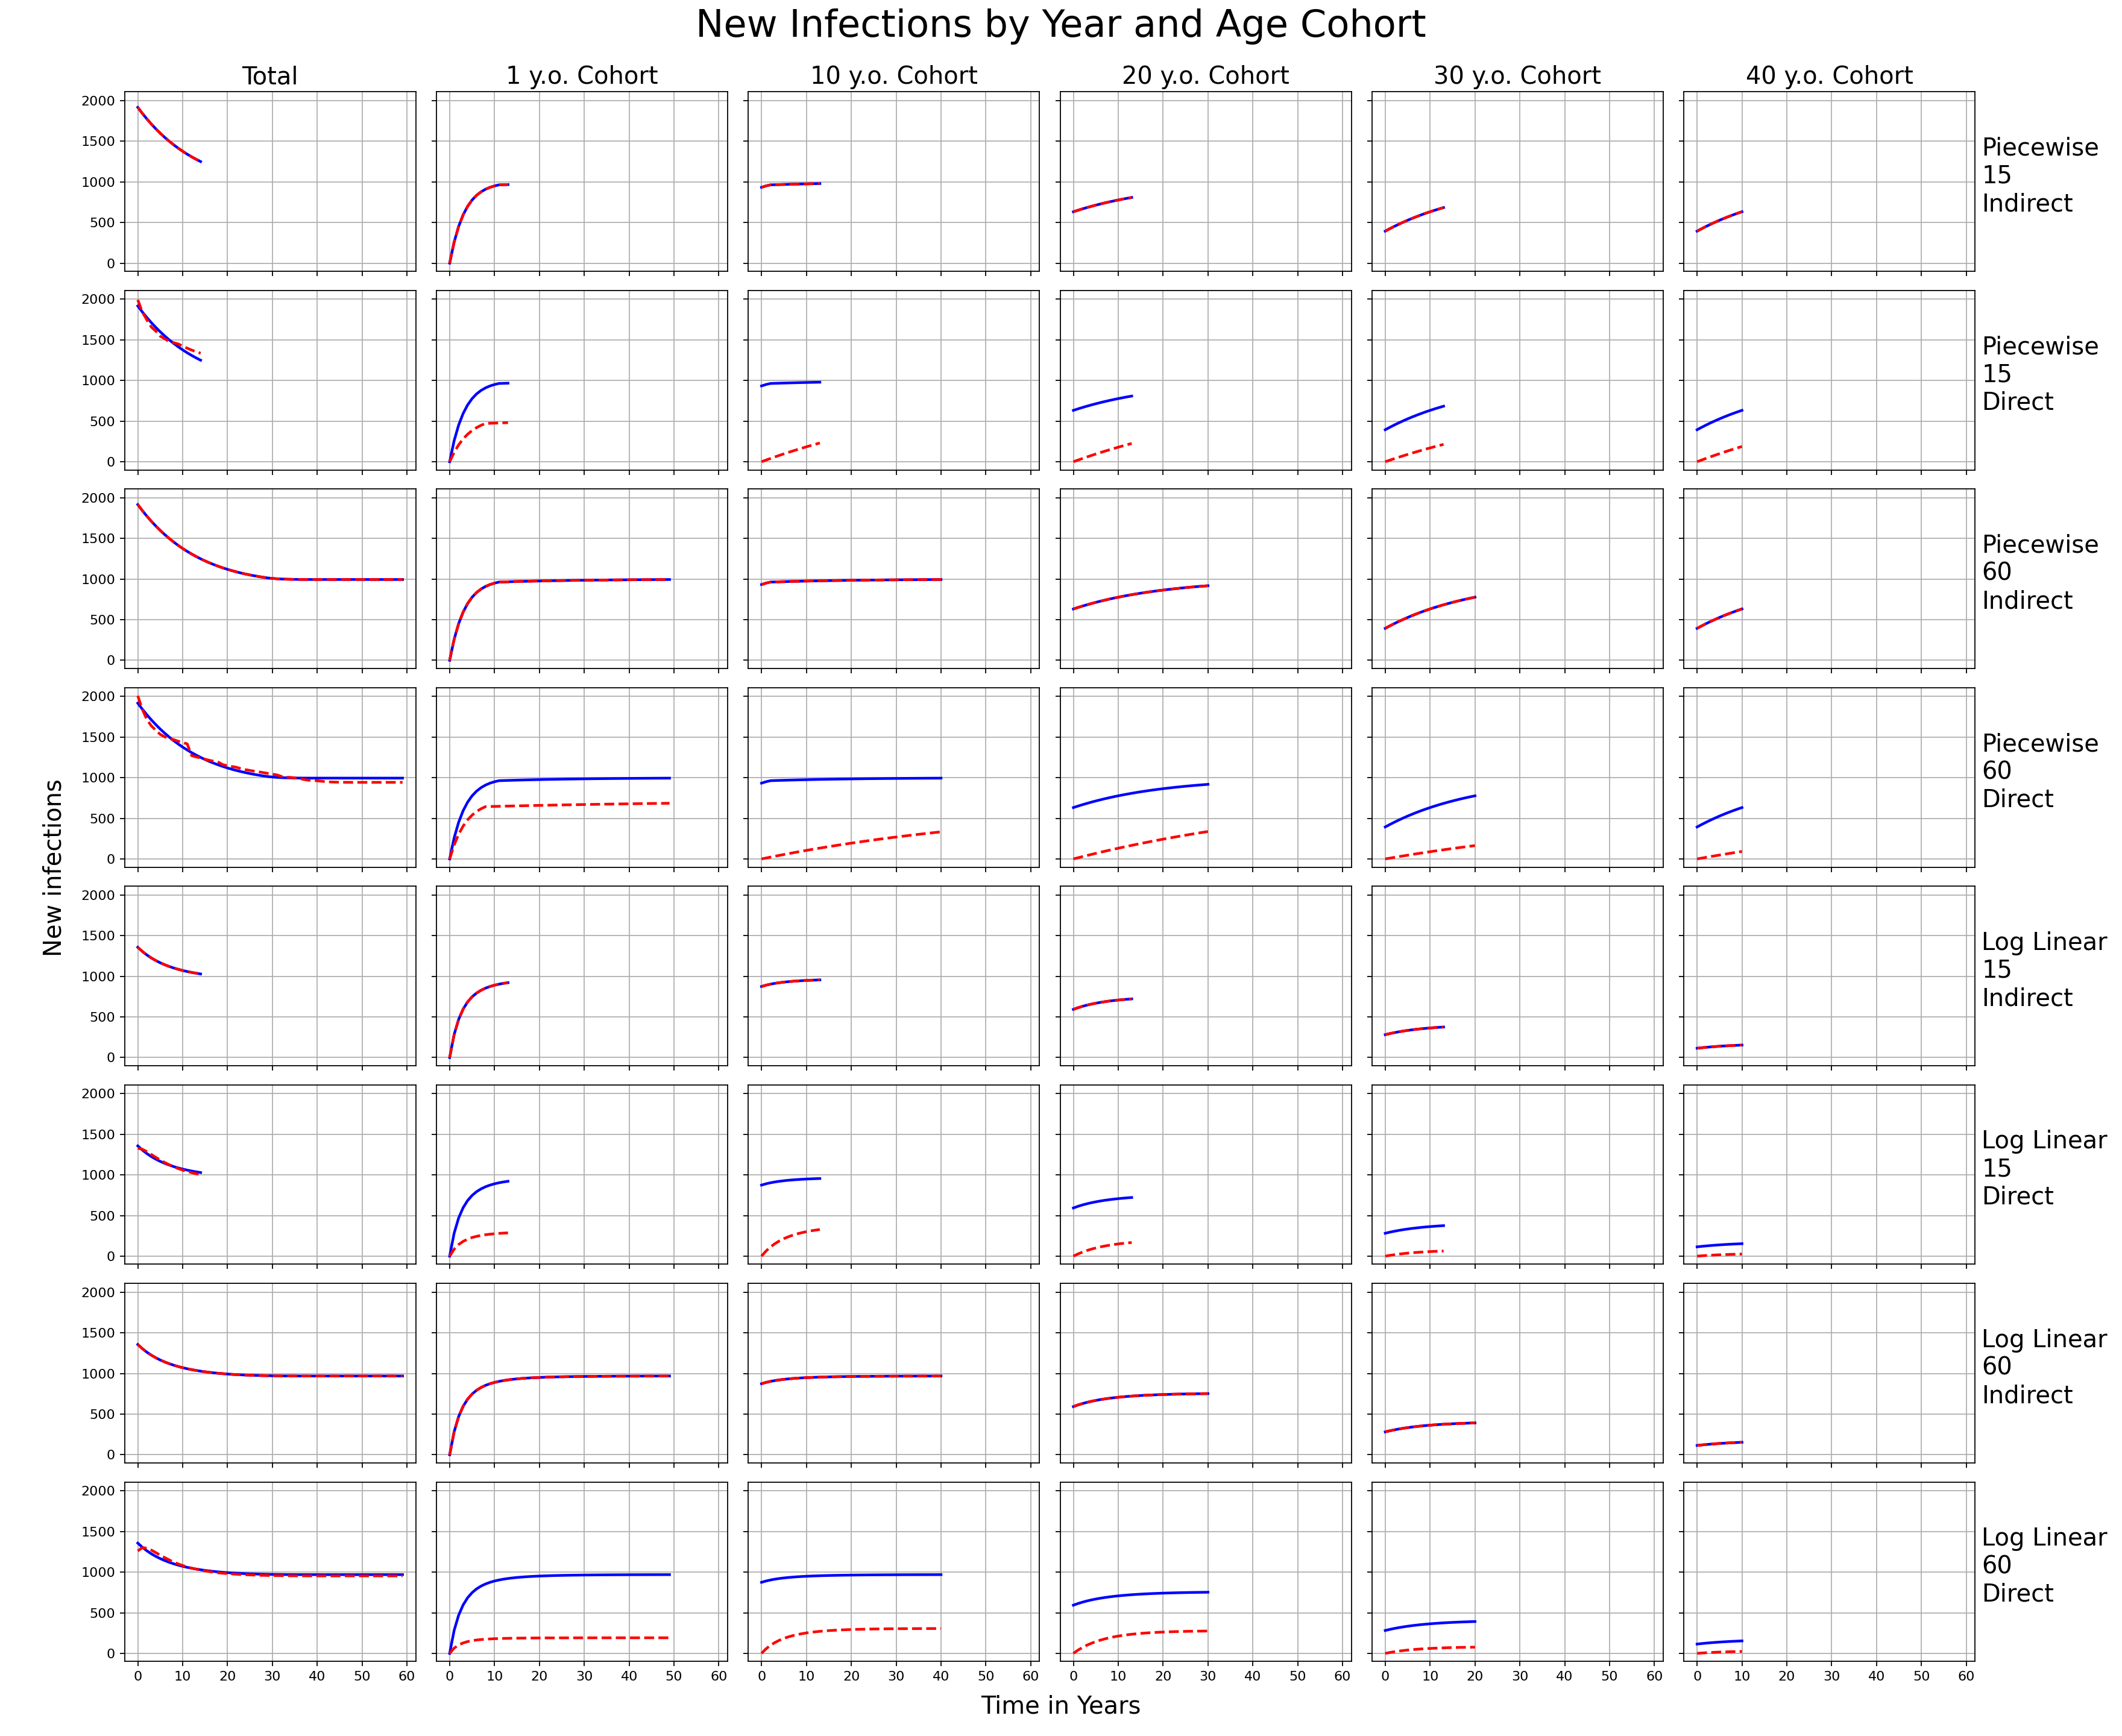
\includegraphics[width=1.15\textwidth]{new_infections_by_year_and_age_cohort.png}
 	\caption{The results of the simulations for various combinations of force of infection form, initializing susceptible and the number of years of data available to the optimization algorithm.}\label{fig:f1}
\end{figure}

\begin{figure}[h]
	\centering
	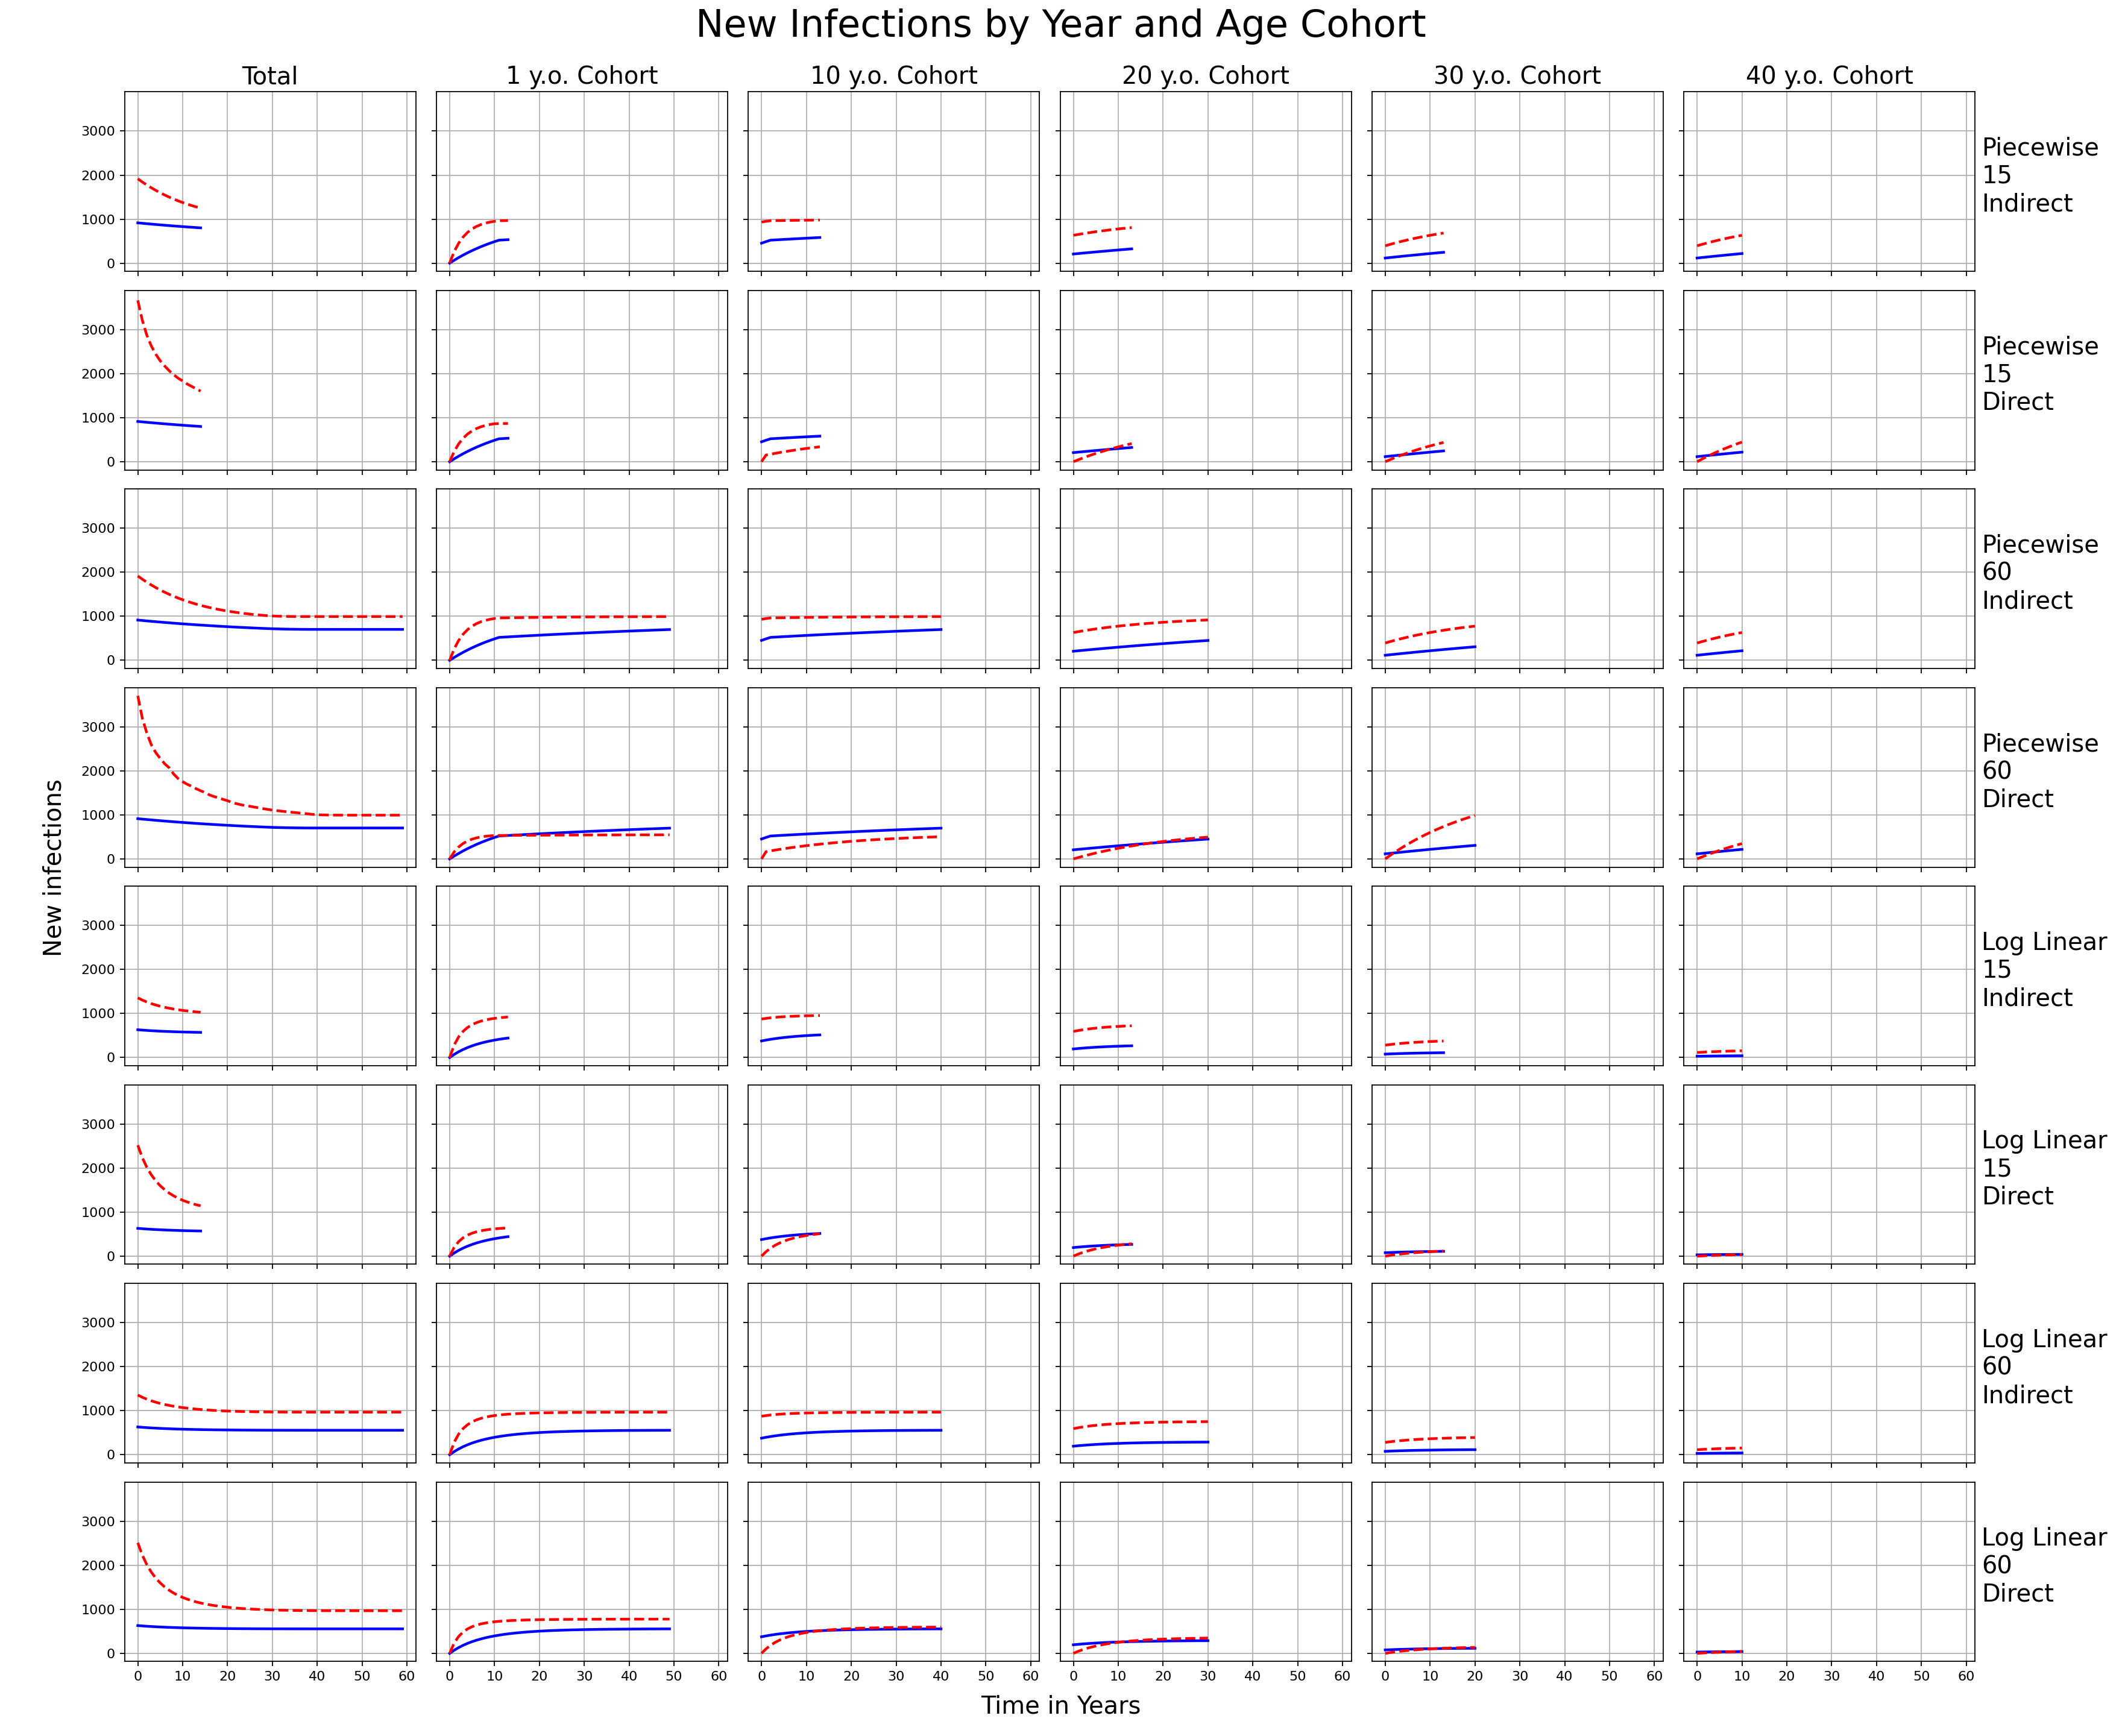
\includegraphics[width=1.15\textwidth]{new_infections_by_year_and_age_cohort_with_rho.png}
 	\caption{The results of the simulations for various combinations of force of infection form, initializing susceptible and the number of years of data available to the optimization algorithm.
	Additionally, this iteration of this adds the $\rho$ parameter for what percentage of infections we actually observe.}\label{fig:f1}
\end{figure}

\end{document}

%%% Local Variables:
%%% mode: latex
%%% TeX-master: t
%%% End:
